\documentclass[12pt,italian]{article}
\usepackage[italian]{babel}
\usepackage[a4paper, margin=1.97cm]{geometry}
\usepackage{graphicx}
\graphicspath{{./images/}}
\usepackage{amsmath}
\usepackage{circuitikz}
\usepackage{caption}
\usepackage{amsfonts}

\usepackage[hidelinks]{hyperref}
\usepackage{cleveref}

\hyphenation{ELVIS}
\newcommand{\err}[1]{\textcolor{red}{#1}}

%\usepackage{fontspec} \setmainfont{calibri}
%\usepackage{titlesec}
%\titleformat{\section}
%{\normalfont\normalsize\itshape}{\thesection.}{1em}{}
%\titlespacing{\section}{0pt}{1em}{0pt}


\title{Misure di grandezze caratteristiche su un circuito crossover}
\author{Enrico Barbuio \\ 0001117553 \and Giacomo Cicala \\ 0001122965} 
\date{\today}

\begin{document}
\maketitle
\section*{Abstract}
L'esperimento ha avuto come obiettivo la progettazione e la realizzazione di un
circuito crossover RLC a tre vie, corredato dallo studio analitico del comportamento in
regime sinusoidale e dal confronto di alcune misure sperimentali con i valori
attesi. Dal punto di vista qualitativo si è osservato che, come previsto, la risposta in
ampiezza del woofer decresce verso zero alle alte frequenze, quella del tweeter
cresce asintoticamente al valore del generatore e il midrange presenta un picco
alla risonanza; le misure di fase confermano la coerenza nella banda passante
ma lo sfasamento fuori banda risulta inferiore a quello atteso. Presentiamo ora
le misure sperimentali affiancate dal valore previsto dalle leggi di Kirchhoff
e dai valori dei componenti.\\ Frequenza di crossover:
\begin{equation*}
	f_{c}^{sper} = (10.61 \pm 0.03) \text{ kHz} \hspace{2cm} f_{c}^{teo} = (10.50
	\pm 0.12) \text{ kHz}
\end{equation*}

\noindent
Frequenza di risonanza:
\begin{equation*}
	f_{r}^{sper} = (10.80 \pm 0.09) \text{ kHz} \hspace{2cm} f_{r}^{teo} = (10.65
	\pm 0.10) \text{ kHz}
\end{equation*}

\noindent
Fattore di qualità del passa-banda del midrange:
\begin{equation*}
	Q^{sper} = 0.88 \pm 0.12  \hspace{2cm}  Q^{teo} = 0.954 \pm 0.010
\end{equation*}

\section*{Introduzione}

L'esperimento svolto in laboratorio è incentrato sulla realizzazione di un
circuito RLC, sullo studio analitico del comportamento atteso e sul confronto
di questo con le misure effettuate.

\begin{figure}
	\centering
	\begin{circuitikz}[scale=1]
		% generatore
		\draw (8,0) --
		(-1,0) --
		(-1,1.5) to[sinusoidal voltage source, label=$v_0$]
		(-1,3) to[R, l=$R_g$, color=blue, bipoles/resistor/height=0.15, bipoles/resistor/width=0.5]
		(-1,4) --
		(-1,5.5) --
		(8,5.5);

		\draw(-1,4.5) to[short, -o]
		(-1.6,4.5) node[left]{$v_g$};
		\draw (-1,1) -- (-1.6,1) node[ground]{};

		% woofer
		\draw (3,5.5) --
		(3,4.5) to[L=$L_w$]
		(3,3.5) to[R, l=$R_{Lw}$, color=blue, bipoles/resistor/height=0.15, bipoles/resistor/width=0.5]
		(3,2.5) --
		(3,2) to[R=$R_w$] (3,0);
		\draw (3,2) to [short, -o] (3.6, 2) node[right]{$v_w$};

		% mid
		\draw (5.5,5.5) to [C=$C_m$]
		(5.5,4.25) to [L=$L_m$]
		(5.5,3.25) to [R, l=$R_{Lm}$, color=blue, bipoles/resistor/height=0.15, bipoles/resistor/width=0.5]
		(5.5,2.25) --
		(5.5,2) to[R=$R_m$] (5.5,0);

		\draw (5.5,2) to [short, -o] (6.1, 2) node[right]{$v_m$};

		%tweeter
		\draw (8,5.5) to[C=$C_t$]
		(8,2) to[R=$R_t$] (8,0);

		\draw (8,2) to
		[short, -o] (8.6, 2) node[right]{$v_t$};
	\end{circuitikz}
	\caption{Schema elettrico del circuito. I punti $v_g, v_w, v_m,
			v_t$ sono stati collegati agli analog input di ELVIS II per le relative
		misure di tensione. I pedici $g$, $w$, $m$, $t$ indicano i rami del generatore, woofer,
		midrange e tweeter. I componenti non ideali sono disegnati in blu.}\label{fig:schema_elettrico}
\end{figure}

Il circuito scelto (\cref{fig:schema_elettrico}) è un crossover a tre vie: un
circuito filtrante che divide un segnale su tre canali al fine di ottimizzare
la riproduzione sonora per tutta la gamma di frequenze. Nel canale del woofer
si trova un filtro passa-basso (RL serie), nel midrange un filtro passa-banda
(RLC serie) e infine nel tweeter un filtro passa-alto (RC serie). I componenti
sono stati scelti per avere la frequenza di risonanza del midrange e la
frequenza di crossover attorno ai $10$ kHz e per far sì che il filtro
passa-banda avesse un fattore di qualità di circa $1$, parametro che verrà poi
verificato sperimentalmente.

Dalla legge di Ohm e dalle leggi di Kirchhoff simboliche per tensioni e
correnti, utilizzando il metodo dei fasori, è stata ricavata la soluzione
stazionaria della differenza di potenziale ai capi del generatore e ai capi
delle resistenze di woofer, midrange e tweeter. Riportiamo qui le loro ampiezze:
\begin{equation}
	\left| \mathbf{V_{g}}(\omega) \right| = \left| 1 - \frac{R_g}
	{\mathbb{Z}_{tot}(\omega)}\right| V_{0}
	\label{eq:Vg}
\end{equation}
\begin{equation}
	\left| \mathbf{V_{w}}(\omega) \right| = \left| \frac{R_{w}}
	{\mathbb{Z}_{w}(\omega)}\right|\left| \mathbf{V_{g}}(\omega) \right|
	\label{eq:Vw}
\end{equation}
\begin{equation}
	\left| \mathbf{V_{m}}(\omega) \right| = \left| \frac{R_{m}}
	{\mathbb{Z}_{m}(\omega)}\right|\left| \mathbf{V_{g}}(\omega) \right|
	\label{eq:Vm}
\end{equation}
\begin{equation}
	\left| \mathbf{V_{t}}(\omega) \right| = \left| \frac{R_{t}}
	{\mathbb{Z}_{t}(\omega)}\right|\left| \mathbf{V_{g}}(\omega) \right|
	\label{eq:Vt}
\end{equation}

\noindent
e le rispettive fasi:
\begin{equation*}
	\phi_{w}(\omega) = Arg(\mathbf{V_{g}}(\omega)) - Arg(\mathbb{Z}_{w}(\omega))
\end{equation*}
\begin{equation*}
	\phi_{m}(\omega) = Arg(\mathbf{V_{g}}(\omega)) - Arg(\mathbb{Z}_{m}(\omega))
\end{equation*}
\begin{equation*}
	\phi_{t}(\omega) =  Arg(\mathbf{V_{g}}(\omega)) - Arg(\mathbb{Z}_{t}(\omega))
\end{equation*}

\noindent
tutto in funzione della pulsazione del generatore e imponendo $\phi_g (\omega) = 0$.

Per quanto riguarda le ampiezze delle tensioni in funzione della frequenza ci
aspettiamo che: il woofer abbia un massimo a basse frequenze e un andamento
decrescente asintoticamente a zero per le alte, il tweeter tenda
asintoticamente al generatore, mentre il midrange dovrà avere un picco alla
frequenza di risonanza. Invece, per quanto riguarda le fasi, woofer e tweeter
dovrebbero essere in fase con il generatore rispettivamente a basse e alte
frequenze, mentre saranno in ritardo e in anticipo di fase di $90^\circ$ nel
caso contrario. Il midrange dovrà essere in fase con il generatore alla
frequenza di risonanza.

Imponendo l'uguaglianza tra le relazioni~\eqref{eq:Vw} e~\eqref{eq:Vt} è
possibile ricavare il valore atteso della frequenza di crossover~\eqref{eq:fc},
cioè la frequenza alla quale il woofer e il tweeter hanno la tensione di
ampiezza uguale.
\begin{equation}
	\label{eq:fc}
	f_{c} = \frac{1}{2\pi}\sqrt{\frac{\sqrt{4 {(R_{w} R_{t} L_{w})}^2 + C_{t}^2{(2
	R_{w} R_{Lw} R_{t}^2 + {(R_{Lw} R_{t})}^2)}^2}}{2 C _{t} {(L_{w} R_{t})}^2 } -
	\frac{R_{w} R_{Lw}}{L_{w}^2} - \frac{R_{Lw}^2}{2 L_{w}^2}}
\end{equation}

Inoltre, da~\eqref{eq:Vm} è possibile calcolare la frequenza di risonanza
attesa del midrange~\eqref{eq:fr} (vedi \cref{sec:resFreq}).

\begin{equation}
	\label{eq:fr}
	f_{r} = \frac{1}{2\pi}\sqrt{\frac{1}{L_{m} C_{m}}}  %equazione approssimata
\end{equation}

Come ultima misura si propone il fattore di qualità del ramo del midrange. Per un
circuito RLC serie questo vale:
\begin{equation*}
	Q =	\frac{1}{R_m}\sqrt{\frac{L_m}{C_m}}
\end{equation*}

\noindent
Sperimentalmente può essere
misurato come:
\begin{equation*}
	Q = \frac{f_r}{\Delta f}
\end{equation*}
con $\Delta f$ larghezza a metà ampiezza della funzione di risposta, o,
equivalentemente, larghezza di banda quando l'ampiezza vale $1/\sqrt{2}$
dell'ampiezza massima.

\section*{Apparato sperimentale e svolgimento}

Il circuito (fig.~\ref{fig:schema_elettrico}) è stato realizzato su una
breadboard. La scheda NI ELVIS II\footnote{NI ELVIS II+ di National
	Instruments. Datasheet:
	\url{https://download.ni.com/support/manuals/372590b.pdf}} è stata utilizzata
come multimetro e dispositivo DAQ unitamente ad un computer dotato di software
apposito all'acquisizione e all'elaborazione delle misure.

I componenti del circuito sono stati misurati tramite il multimetro di ELVIS
II, i loro valori e le rispettive incertezze (strumentali) si trovano in
\cref{tab:componenti}.

\begin{table}[h]
	\begin{alignat*}{6}
		 & R_w                               &  & =(3293 \pm 2) \text{ \Omega} \hspace{2cm} &  & R_m    &   & =(3287 \pm 2) \text{ \Omega} \hspace{2cm} &  & R_t &  & =(3295 \pm 2) \text{ \Omega}      \\
		 & L_w                               &  & =(47.1 \pm 0.5) \text{ mH}                &  & L_m    &   & =(46.8 \pm 0.5) \text{ mH}                &  & C_t &  & =(4.68 \pm 0.05) \text{ nF}       \\
		 & R_{Lw}                            &  & =(120.00 \pm 0.15) \text{ \Omega}         &  & R_{Lm} &
		 & =(120.70 \pm 0.15) \text{ \Omega} &  &                                           &  &                                                                                                        \\
		 &                                   &  &                                           &  & C_m    &   & =(4.76 \pm 0.05) \text{ nF}               &  & R_g &  & =50 \text{ \Omega \ (dichiarata)}
	\end{alignat*}
	\caption{Valori dei componenti del circuito.} \label{tab:componenti}
\end{table}

Per l'analisi in frequenza di ampiezza e fase è stato acquisito ciascun canale
separatamente, con sweep ripetuti. In ogni misura l'analog input \texttt{A1} è
stato collegato al canale di interesse mentre il canale \texttt{A0} è rimasto
sempre collegato al generatore di tensione, utilizzandolo come trigger e
riferimento per la fase. Al fine di massimizzare la
frequenza di campionamento, le tensioni sono state misurate in modalità
referenced single ended collegando a massa il ramo in comune alle resistenze.
Ciò ha permesso un campionamento a $500$ kHz per canale, con $2000$ sample per
ciascuna acquisizione, abbastanza per includere almeno $4$ periodi a qualsiasi
frequenza del range. Dalle differenze di tensione acquisite nel dominio dei
tempi sono state estratte automaticamente fasi e ampiezze in funzione della
frequenza. Per gli sweep è stato scelto un range di frequenze di
$1$ kHz - $50$ kHz, questo per evidenziare il punto di crossover ma anche per
vedere l'andamento a basse e alte frequenze.

\section*{Risultati e discussione}
Dalle misure delle componenti riportate in \cref{tab:componenti} e
dall'equazione~\eqref{eq:fc} abbiamo ricavato la frequenza di crossover:
\begin{equation*}
	f_{c}^{teo} = (10.50 \pm 0.12)\  \text{ kHz} \hspace{2cm} \frac{\Delta f_{c}}{f_{c}} = 1.1 \ \%
\end{equation*}

\noindent
Analogamente, la frequenza di risonanza del midrange attesa è risultata:
\begin{equation*}
	f_{r}^{teo} = (10.65 \pm 0.11)\  \text{ kHz} \hspace{2cm} \frac{\Delta f_{r}}{f_{r}} = 1.0 \ \%
\end{equation*}
Quest'ultimo valore fa fede alla relazione ideale~\eqref{eq:fr} perché gli effetti del circuito reale sono risultati inferiori
all'errore strumentale, più dettagli in \cref{sec:resFreq}. Entrambe le incertezze sono state propagate linearmente e sono da considerarsi assolute.

Per ricavare $f_{c}$ e $f_{r}$ dalle misure di ampiezza, si sono eseguiti dei
fit (\cref{fig:amp_sweep}) in un intorno ristretto delle due frequenze
interessate ($ 7 $ kHz - $ 14 $ kHz) con le funzioni (\ref{eq:Vg}),
(\ref{eq:Vw}), (\ref{eq:Vm}) e (\ref{eq:Vt}). Le incertezze associate ai punti
sperimentali sono:
\begin{equation*}
	\Delta V = 1.9 \text{ mV} \hspace{2cm} \Delta f = 0.186 \text{ Hz}
\end{equation*}

\noindent
il primo è l'errore di risoluzione degli analog input di ELVIS; il secondo
deriva dalla precisione del generatore sinusoidale, l'unico riferimento per
le nostre misure di frequenza. Riportiamo di seguito i $\tilde{\chi}^2$ dei fit:
\begin{equation*}
	\tilde{\chi}^2_{g} = 1.05  \hspace{1cm} \tilde{\chi}^2_{w} = 0.562 \hspace{1cm} \tilde{\chi}^2_{m} = 0.868 \hspace{1cm} \tilde{\chi}^2_{t} = 0.927
\end{equation*}

\begin{figure}[h]
	\centering
	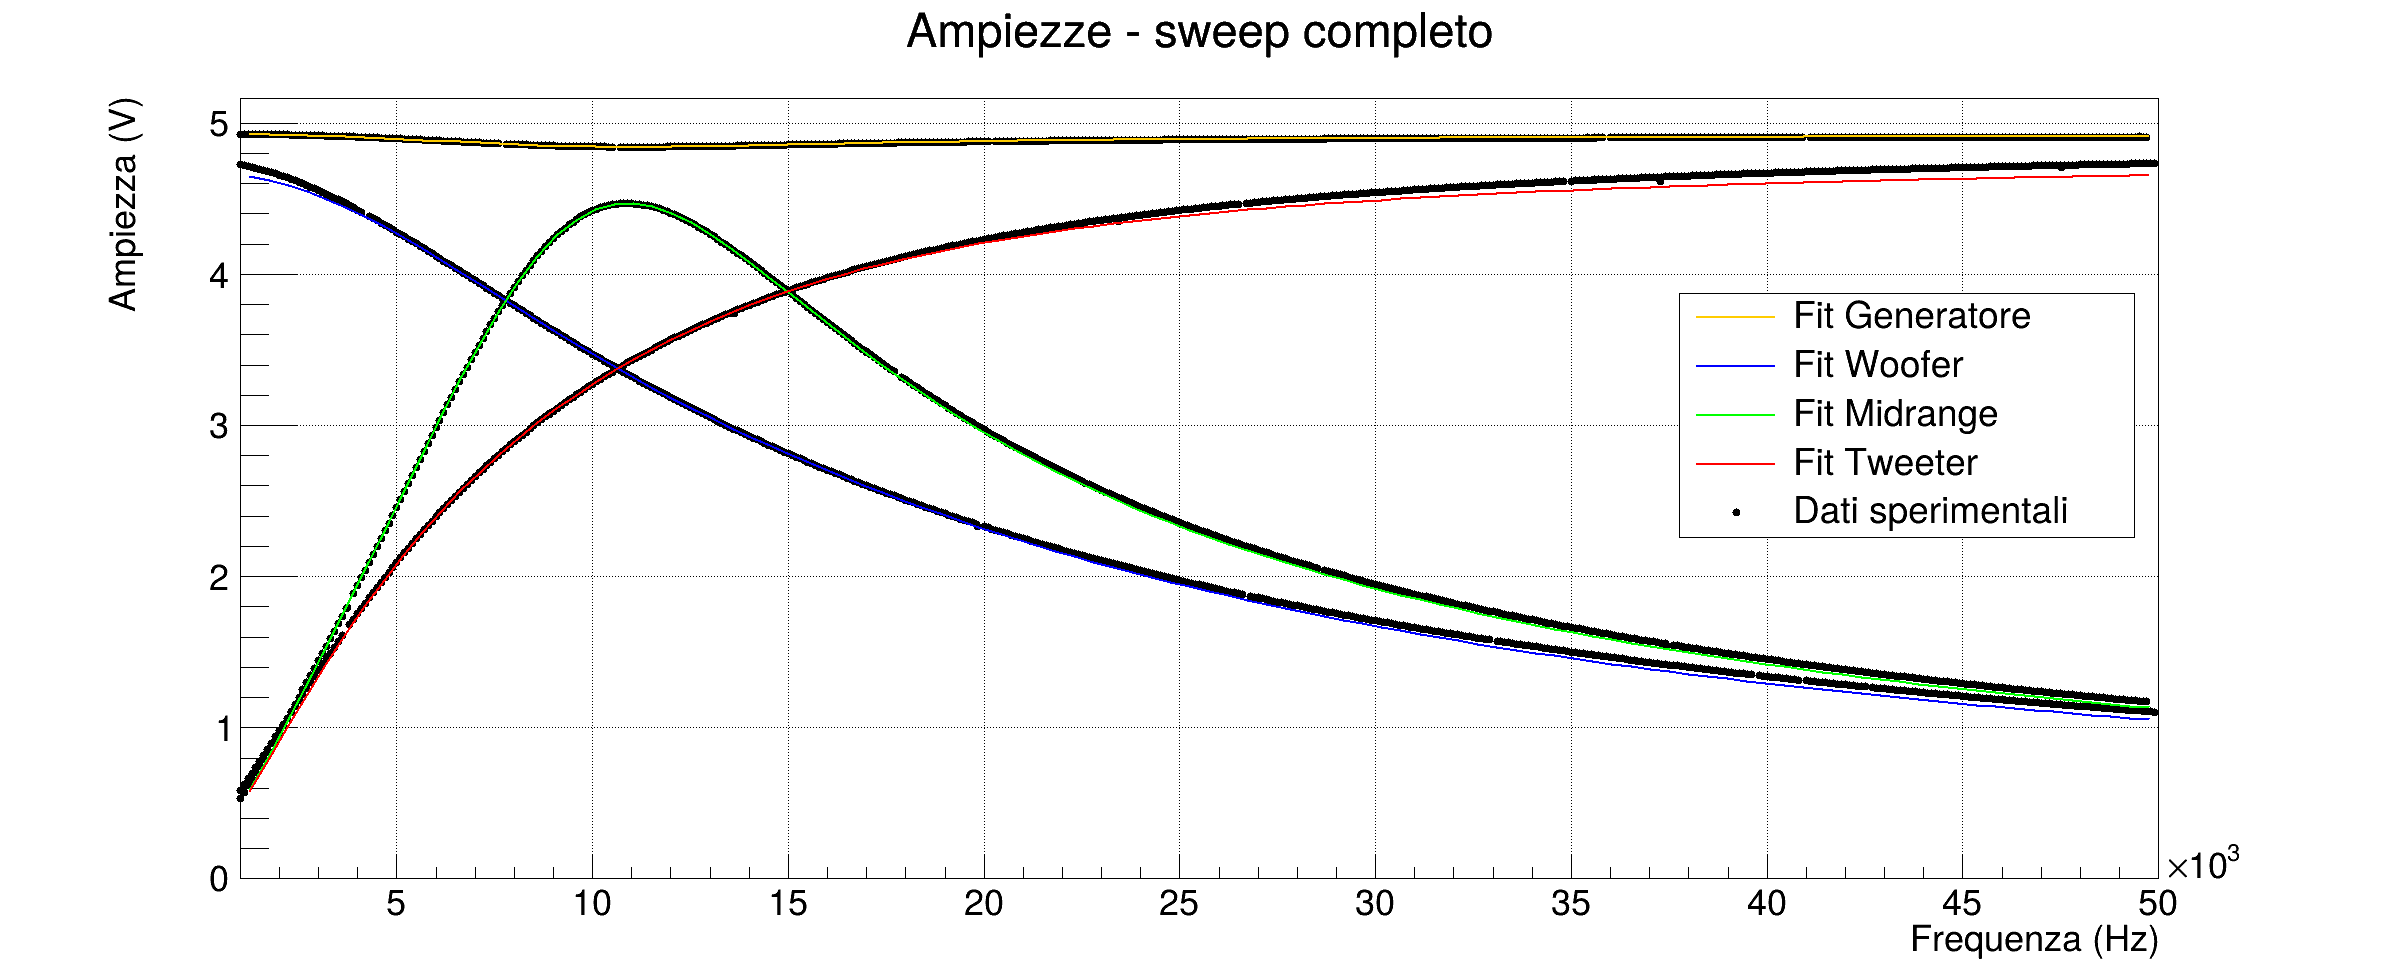
\includegraphics[width=\textwidth]{fig_amp.png}
	\caption{Grafico delle ampiezze delle tensioni in funzione della frequenza per il woofer, midrange, tweeter e generatore. I fit sono eseguiti nell'intervallo $7$ kHz - $14$ kHz e le funzioni risultanti graficate su tutto il range di acquisizione.}\label{fig:fc_fr}
	\label{fig:amp_sweep}
\end{figure}

Dai dati sperimentali delle ampiezze, $f_{c}$ è stata misurata uguagliando
numericamente le funzioni del woofer e del tweeter. $f_{r}$ è stata calcolata
come frequenza corrispondente al massimo della funzione di fit. Le incertezze
sono state propagate in quadratura a partire dai parametri del fit e vanno
considerate come statistiche.
\begin{equation*}
	f_{c}^{amp} = 10.64 \text{ kHz} \hspace{2cm} \sigma_c^{amp} = 0.02 \text{ kHz}
\end{equation*}
\begin{equation*}
	f_{r}^{amp} = 10.89 \text{ kHz} \hspace{2cm} \sigma_r^{amp} = 0.16 \text{ kHz}
\end{equation*}

Per verificare le proprietà filtranti del circuito è possibile svolgere
un'analisi qualitativa delle ampiezze per il range di frequenze complessivo
acquisito: dalla (\cref{fig:fc_fr}) si può notare, come ci aspettavamo, che
woofer, midrange e tweeter si comportano rispettivamente come un filtro
passa-basso, un passa-banda e un passa-alto; tuttavia si osserva che il modello
da noi utilizzato non si adatta ai dati sperimentali per range di frequenze
così ampi.

Le misure di fase in funzione della frequenza presentavano una deriva
sistematica. Questa è dovuta al fatto che nell'acquisizione il multiplexer
della scheda impiega $1$ \textmu{s} a cambiare canale da \texttt{A0} a
\texttt{A1}, generando uno sfasamento proporzionale alla frequenza analizzata.
Per correggerla si è eseguito un fit della fase del generatore sul canale
\texttt{A1}, sottraendola poi al grafico di ciascun canale. Inoltre per
eliminare la dipendenza dal trigger i valori delle fasi non sono assoluti ma
ottenuti sempre come differenza tra fase di \texttt{A1} e di \texttt{A0}; in
questo modo la deviazione standard sulle misure di fase è $\sigma_\phi =
	0.003^\circ$ su tutto il range di frequenze. Nonostante queste correzioni, i
punti sperimentali (\cref{fig:phase_sweep}) si sono discostati parecchio dalla
funzione attesa, specialmente sotto i $7$ kHz e sopra i $25$ kHz. Data la
complessità del modello non siamo riusciti a ottenere un fit convergente
neanche su regioni ristrette, di conseguenza non abbiamo potuto associare un
incertezza significativa alle misure ricavate in questo modo.
\begin{equation*}
	f_{c} = 10.601 \text{ kHz} \hspace{2cm} f_{r} = 10.791 \text{ kHz}
\end{equation*}

\noindent
Si è deciso allora di approssimare localmente (nell'intervallo $10$ kHz -
$11.2$ kHz) il grafico delle fasi con una retta. In questo modo abbiamo
misurato:
\begin{equation*}
	f_{c}^{fasi} = 10.600 \text{ kHz}  \hspace{2cm}  \sigma_c^{fasi} = 0.010 \text{ kHz}
\end{equation*}
\begin{equation*}
	f_{r}^{fasi} = 10.80 \text{ kHz}  \hspace{2cm}  \sigma_r^{fasi} = 0.03 \text{ kHz}
\end{equation*}

\begin{figure}[h]
	\centering
	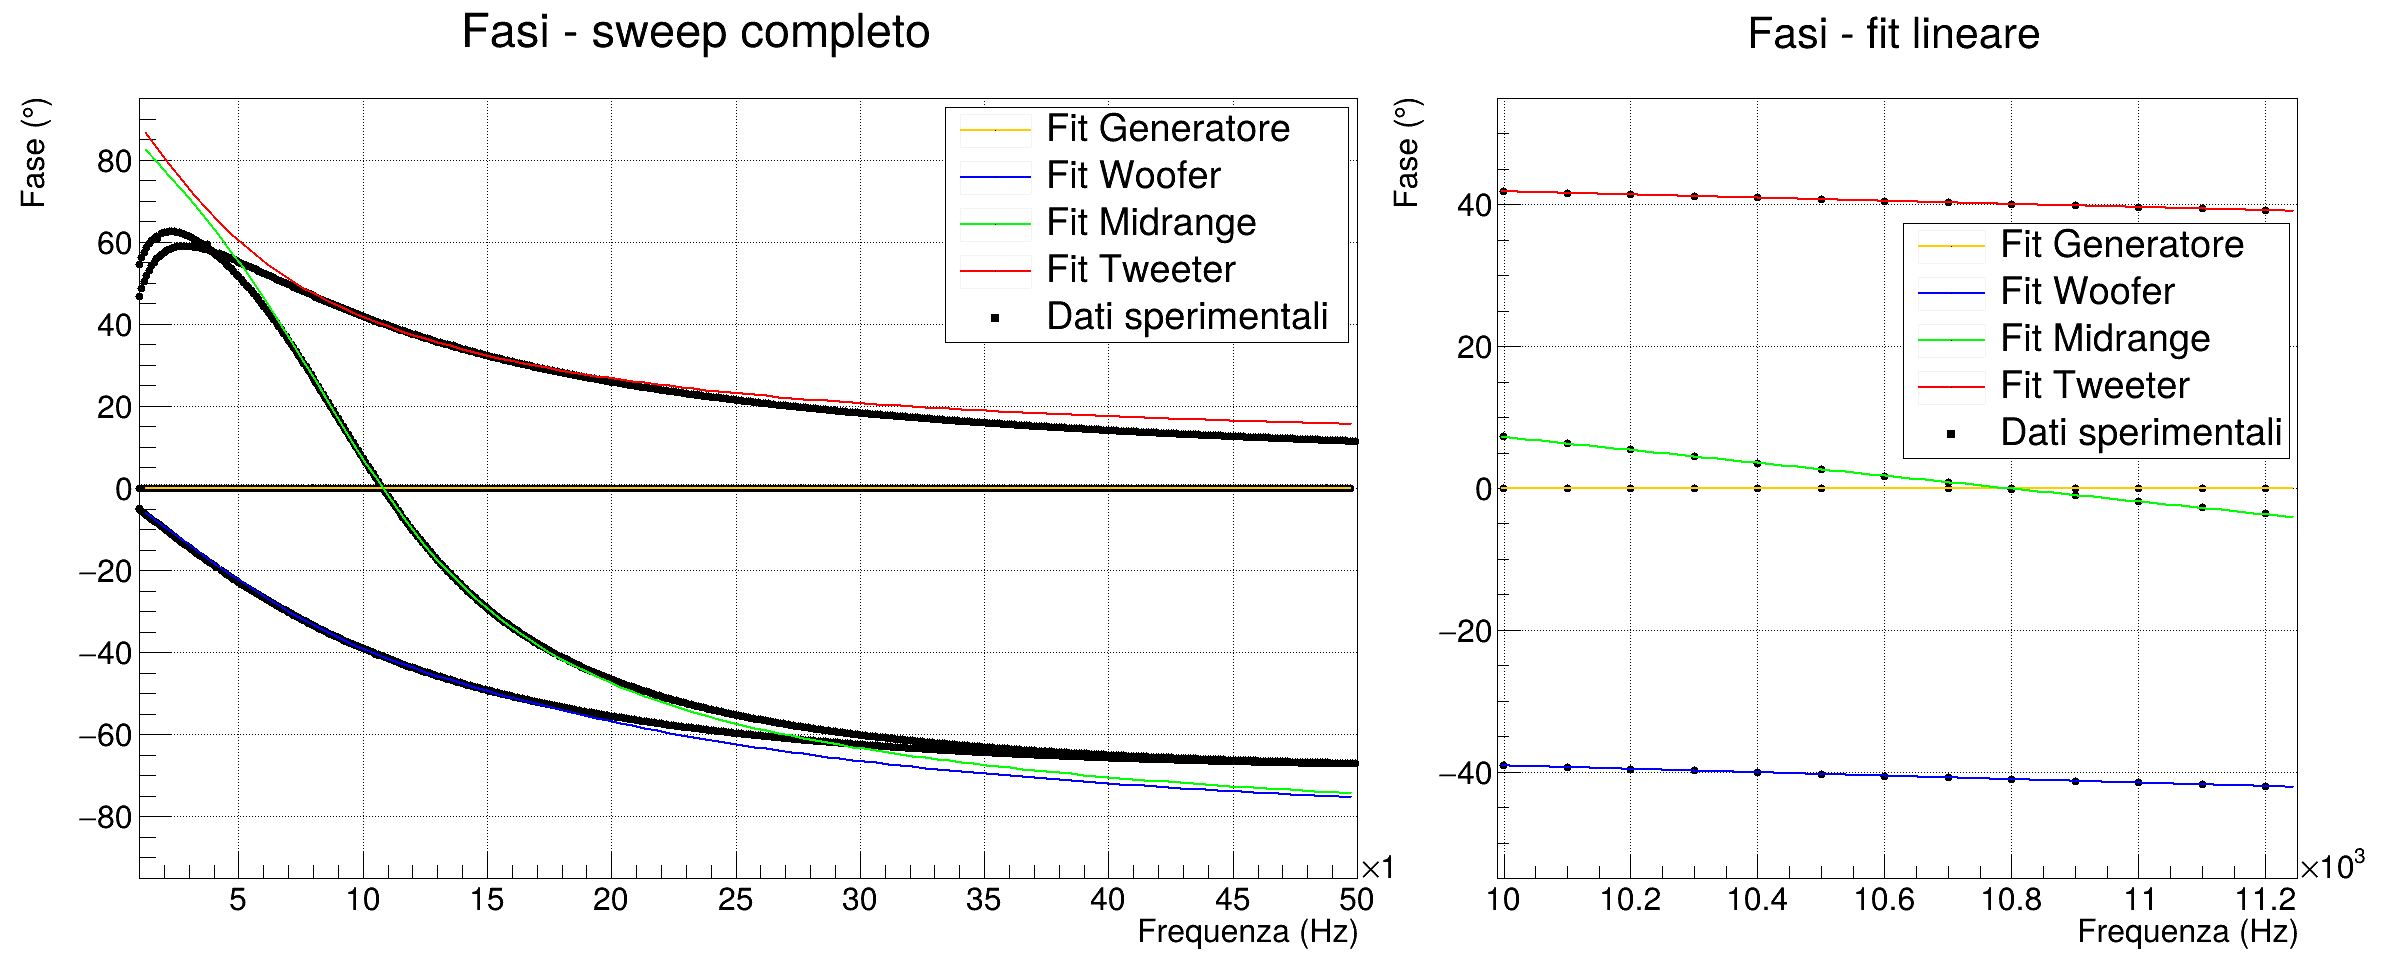
\includegraphics[width=\textwidth]{fig_fase.png}
	\caption{A sinistra: grafico delle fasi in funzione della frequenza per il woofer, midrange, tweeter e generatore;
		fit ristretto al range $8$ kHz - $16$ kHz, funzione estesa a tutto il dominio dei dati. A destra: fit lineare degli stessi dati da $10$ kHz a $11.2$ kHz.}\label{fig:phase_sweep}
\end{figure}

La media pesata delle due misure sperimentali è:
\begin{equation*}
	f_{c}^{sper} = 10.608 \text{ kHz}  \hspace{2cm}  \sigma_c^{sper} = 0.009 \text{ kHz}
\end{equation*}
\begin{equation*}
	f_{r}^{sper} = 10.80 \text{ kHz}  \hspace{2cm}  \sigma_r^{sper} = 0.03  \text{ kHz}
\end{equation*}

\noindent
Assumendo che le incertezze statistiche provengano da una popolazione
gaussiana, utilizziamo un fattore di copertura $k = 3$ per ottenere un
$\text{C.L.}\approx 99 \ \% $ e trattare le incertezze come assolute. Otteniamo
dunque
\begin{equation*}
	f_{c}^{sper} = (10.61 \pm 0.03) \text{ kHz} \hspace{2cm} \frac{\Delta f_{c}^{sper}}{f_{c}^{sper}} = 0.3 \ \%
\end{equation*}
\begin{equation*}
	f_{r}^{sper} = (10.80 \pm 0.09) \text{ kHz} \hspace{2cm} \frac{\Delta f_{r}^{sper}}{f_{r}^{sper}} = 0.8 \ \%
\end{equation*}

\noindent
Poiché gli intervalli di incertezza delle due stime sperimentali si
sovrappongono a quelli delle rispettive stime teoriche, possiamo affermare che
queste risultano compatibili.

Infine sul canale del midrange è stato misurato il fattore di qualità. Dai
parametri del circuito ci si aspetta:
\begin{equation*}
	Q^{teo} = 0.954 \pm 0.010
\end{equation*}
mentre sperimentalmente:
\begin{equation*}
	Q^{sper} = 0.88 \pm 0.12
\end{equation*}
sempre considerando un fattore di copertura $3$.

\section*{Conclusioni}

Dunque, per la frequenza di crossover, per quella di risonanza e per il fattore
di qualità del midrange abbiamo ottenuto due stime, una teorica e una
sperimentale, compatibili tra loro.
\begin{equation*}
	f_{c}^{sper} = (10.61 \pm 0.03) \text{ kHz} \hspace{2cm}
	f_{c}^{teo} = (10.50 \pm 0.12) \text{ kHz}
\end{equation*}
\begin{equation*}
	f_{r}^{sper} = (10.80 \pm 0.09) \text{ kHz}
	\hspace{2cm} f_{r}^{teo} = (10.65 \pm 0.10) \text{ kHz}
\end{equation*}
\begin{equation*}
	Q^{sper} = 0.88 \pm 0.12 \hspace{2cm} Q^{teo} = 0.954 \pm 0.010
\end{equation*}

Gli andamenti delle ampiezze sono stati coerenti con le aspettative, ovvero si
sono osservati i comportamenti di un filtro passa-basso per il woofer, un
filtro passa-banda per il midrange e un filtro passa-alto per il tweeter.
Tuttavia, pur tenendo conto degli effetti non ideali dei componenti, il modello
non è esatto su tutto il range di frequenze ma risulta compatibile con i dati
solamente in un intervallo ristretto ($7$ kHz - $14$ kHz).

Invece, l'andamento delle fasi si è discostato in maniera significativa dal
comportamento atteso. Per tweeter e midrange, sotto i $6$ kHz si osserva una
decrescita anomala che non siamo riusciti a spiegare. Mentre sulle alte
frequenze i dati hanno un asintoto diverso da quello previsto.

\appendix
\section{Appendici}
\subsection{Frequenza di risonanza}\label{sec:resFreq}
La prima misura è data dalla relazione ideale~\eqref{eq:fr}, la seconda tiene
conto anche degli effetti non ideali ed è stata ricavata numericamente come
frequenza corrispondente al massimo dell'equazione~\eqref{eq:Vm}.
\begin{equation*}
	f_{r}^{\text{(ideale)}} = 10652 \text{ Hz} \hspace{2cm} f_{r}^{\text{(reale)}} = 10651 \text{ Hz}
\end{equation*}
% f_r
Poiché l'errore percentuale che si commette prendendo $f_{r}^{\text{(ideale)}}$
come miglior stima è solamente $\varepsilon_{f_r} \approx 0.01\%$, si è scelto
di utilizzare questa stima per poter propagare con semplicità l'incertezza, che
risulta essere
\begin{equation*}
	\begin{alignedat}{2}
		\frac{\Delta f_{r}}{f_{r}} = & \frac{1}{2} \frac{\Delta L_{m}}{L_{m}} &  & + \frac{1}{2} \frac{\Delta C_{m}}{C_{m}} \\
		=                            & 0.0050                                 &  & + 0.0050
		= 0.010 = 1.0 \ \%
	\end{alignedat}
\end{equation*}
ossia due ordini di grandezza maggiore di $\varepsilon_{f_r}$
\end{document}
